% Bài giảng Khoa học tự nhiên 9 - Khúc xạ ánh sáng
\section{Hiện tượng khúc xạ ánh sáng}

\subsection{I. Định nghĩa khúc xạ ánh sáng}
Hiện tượng tia sáng truyền từ môi trường trong suốt này sang môi trường trong suốt khác bị gãy khúc tại mặt phân cách giữa hai môi trường gọi là hiện tượng khúc xạ ánh sáng.

Hình học khúc xạ qua hình vẽ TikZ:
\begin{center}
\begin{tikzpicture}[scale=0.9]
\draw[thick, blue] (-3,0) -- (3,0) node[right] {Mặt phân cách};
\draw[dashed] (0,-2) -- (0,2) node[above] {$N N'$ (Pháp tuyến)};
\draw[->, red, very thick] (-2,1.5) -- (0,0) node[midway, above left] {Tia tới $SI$};
\draw[->, red, very thick] (0,0) -- (1.2,-1.6) node[midway, below right] {Tia khúc xạ $IR$};
\node at (-1.8,0.8) {Không khí};
\node at (-1.8,-0.8) {Nước};
\end{tikzpicture}
\end{center}

Hình ảnh thực nghiệm:
\begin{center}
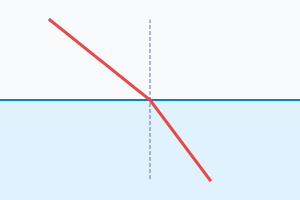
\includegraphics[width=0.6\linewidth]{images/refraction_diagram.png}
\par\textit{Hình 1: Mô phỏng khúc xạ ánh sáng khi truyền từ không khí vào nước}
\end{center}

\subsection{II. Câu hỏi trắc nghiệm}

\begin{ex}
Chiếu một tia sáng từ không khí vào nước với góc tới $i = 60^\circ$. Đánh giá tính đúng/sai của các nhận định sau:
\choiceTF
{\True Tia sáng truyền vào nước và bị lệch phương so với tia tới}
{\True Góc khúc xạ $r$ nhỏ hơn góc tới $i$}
{Tia sáng luôn đi thẳng không đổi phương}
{Góc khúc xạ $r$ luôn lớn hơn góc tới $i$}
\loigiai{
Khi ánh sáng truyền từ không khí sang nước (môi trường chiết quang hơn), tia khúc xạ bị bẻ cong về phía pháp tuyến, do đó $r < i$.
}
\end{ex}
